\documentclass[onecolumn]{paper}
\usepackage{tabularx}
\usepackage{color}
\usepackage{listings}
\usepackage{verbatim}
\usepackage{quiver}
\usepackage{caption}
\usepackage{subcaption}

\newcolumntype{L}{>{\raggedright\arraybackslash}X}

\title{ConFrm: Confidentiality Framework for Crash Safe Storage Systems}
\author{Atalay Mert Ileri \and Frans Kaashoek \and Nickolai Zeldovich}

\begin{document}
\maketitle
\chapter{Introduction}

Explain the reason why there are two and how they compare to each other.



%% TODO: Short intro here
\subsection{Threat Model}
% Taken and tweaked from disksec
From the perspective of verification, we would like to have confidence
that the file system is secure purely based on the file system's security
specification.  This means that we have to treat the developer of the
file system with an adversarial mindset.  This subsumes all possible
bugs that a well-meaning but error-prone developer might introduce into
the implementation as well as any implementation that is designed to be exploited.

As a result, our threat model is that the adversary both develops the
file system and runs an adversarial application on top of the file system
in an attempt to obtain confidential file data.  However, the adversary
does provide a proof that their file-system implementation meets our
security specification.  The potential victim runs on top of the same
file system but sets their permissions so that the confidential files
are not accessible to the adversary's process.  Our goal is to ensure
that the security specification is so strong that it prevents leaks even
when the file-system developer is colluding with adversarial processes
running on top of the file system.

Our threat model is focused on proving that the file-system implementation has
no confidentiality bugs, rather than proving the absence of bugs in the
environment outside of the file system. Thus, we assume that our model
of how the file-system implementation executes is correct.  That is, we are not
concerned with bugs in unverified software or hardware outside of the file
system, or users mounting malicious disk images.  We do prove that
\texttt{mkfs} produces a correct image, but ensuring confidentiality on top of an
intentionally corrupted file system image is difficult, even without formal
verification. 

%%% Disksec doesn't reason about time. ConFrm reasons about it at coarse granularity.
%%% TODO: I will add these to their respective chapters

%We also do not reason about timing channels, as we do not model time.

%We only reasoning about time in a coarse granularity, 
%i.e. number of operations executed. Each operation having having different execution time 
%(e.g. a memory write is much faster than a disk write) is out of scope of this work.


% Taken from disksec
\subsection{Challenges}
\label{s:goal:chal}

The most difficult aspect of formally proving the security of a file system lies
in guaranteeing confidentiality.  This is difficult for several reasons.

\paragraph{Two-safety.}
First, proving confidentiality is more difficult than
proving functional correctness: as mentioned earlier, confidentiality
is a two-safety property.  Functional correctness is a one-safety
property because a violation of functional correctness can be demonstrated
by a single execution.  For instance, if an application wrote one byte to
a file and then read back a different byte, this single execution shows
that the file system is incorrect.  Thus, functional correctness
of a file system is a theorem that says that all executions meet the
spec (i.e., there are no such violations).  Integrity properties,
such as ensuring that one user cannot corrupt another user's data,
are an example of a one-safety functional-correctness property and can
be handled using standard verification techniques.

In contrast, demonstrating a violation of confidentiality requires
two executions, where the results observed by an adversary differ depending on
the secret data.
%% %% TODO: We don't do this though. Maybe find a better example for this?
For instance, consider a file system with block-level deduplication that
also exposes the number of free blocks.  An adversary who wants to
learn the contents of a victim's file could write their guess for the
victim's block into the adversary's own file and then check whether
the number of free blocks stayed the same or decreased.  If the file
system implemented deduplication across users, this attack allows an
adversary to learn whether their guess block was already present in the
file system, thus inferring whether the victim has that data.

In the above example, looking at a single execution does not allow one
to directly conclude that data was leaked, because the system appears
to be functioning correctly.  Determining that data is leaking requires
one to consider a pair of executions, in which the adversary performs
the same operations, but the confidential user data is different.
If these two executions produce different adversary-observable results,
the adversary is able to infer information about confidential data.

By stating confidentiality as a two-safety property, the above
deduplication example would violate confidentiality, and thus could not
appear in an implementation that was proven to achieve confidentiality.
Specifically, suppose the starting states of the two executions differed
in the contents of a confidential file, where in one execution the file
matched the adversary's guess and in the other execution it didn't match.
In this case, the number of free blocks returned by the adversary
would differ in the two executions, which would not be allowed by the
confidentiality definition.

\paragraph{Nondeterministic specifications.}
Another complication in proving confidentiality lies in the fact
that many specifications, including those in the file system, are
nondeterministic.  Some nondeterminism is unavoidable because file
systems must deal with crashes (e.g., due to power failure), which can
occur at any time.  Thus, it is impossible to
know what are the exact contents of the disk after a crash; the on-disk
state could reflect any prefix of the writes issued by the file system.
Modern disks complicate this situation even further by buffering writes
in memory inside the disk controller; as a result, the writes can be
made durable out-of-order, and the state of the disk after a crash might
reflect some out-of-order writes.  Even in the absence of crashes, the
file system implementation may want to use randomness (e.g., to randomize
directory hash tables), which makes the execution non-deterministic.

Other nondeterminism comes from specifications that hide irrelevant
details.  For instance, the inode allocator in the file system does
not specify which precise inode number will be returned; instead,
its specification simply states that it will return
\emph{some} inode number that is not already in use.

Any nondeterminism is a potential leak of confidential data.  The
nondeterministic specification of the block allocator from above does not
preclude the allocator from leaking confidential data, because it could,
in theory, choose the next inode number based on the confidential contents
of files, without violating its specification (i.e., still returning some
unused inode number).

Even the nondeterminism associated with the state of the disk
after a crash can be taken advantage of by an adversarial file-system
implementation to leak data.  For instance, a high-performance
file-system specification allows the file system to delay flushing data
to disk.  An adversarial implementation could choose whether to flush
data immediately or defer the flush based on one bit of confidential
data from a victim's file.  To take advantage of this, an adversary
could wait for the system to crash and, after the crash, check whether
any writes appear to have been lost.  If so, the adversary concludes
the file system must have deferred the writes, which would have only
happened if the confidential bit was zero.  This, in turn, can allow
the adversary to infer confidential bits.

\paragraph{Non-uniform outcome probabilities.}
Another possibility of leaking confidential data
arises because standard nondeterministic noninterference
captures what \emph{might} be possible, but an adversary may have
more precise information about the actual \emph{probabilities} of
different outcomes. A simple example of this weakness can be seen below: 

\begin{figure}[ht]
    \centering
\begin{verbatim}
if (random_bit() = 1)
  return secret_bit
else
  return random_bit()
\end{verbatim}
    \caption{Example of a noninterfering program that leaks information via return value frequencies}
    \label{fig:Frequency_Leaking_Program}
\end{figure}

This code leaks the secret bit 50\% of the time and outputs a random bit 50\% of the time. It is also important to note that it can output 0 or 1 independently of the secret value. This way, any (state, return) pair represents a successful execution. 

Let’s say that two states are equivalent if they are the same for their non secret parts. This makes all states equivalent to each other in our example. Since any pair of state and return value is a valid execution, it is possible to find another execution from a related state with same return value. Therefore, This implementation satisfies the nondeterministic noninterference definition. 

\begin{figure}[ht]
    \centering
    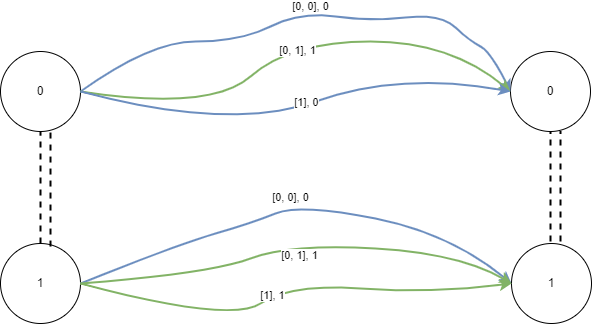
\includegraphics[scale=0.5]{templates/figures/matching-paths.png}
    \caption{Every execution matches with the execution of the same color.\\
    Numbers in brackets denote generated random bits. \\The number following the brackets denotes the return value.}
    \label{fig:NI_Matching_Paths}
\end{figure}

Although the above program satisfies the definition, the secret bit can be determined via the observed frequency of repeated calls. When we look at the frequencies of output values, we can see that they correlate with the value of the secret bit. \\

\begin{tabular}{| c | c | c |}
	\hline
	Secret bit & Output 0 \% & Output 1 \% \\
	\hline
	0 &	75\% & 25\% \\
	\hline
	1 &	25\% & 75\% \\
	\hline
\end{tabular}\\

Any adversary who can observe the output of the function sufficiently many times can infer the value of the secret bit with high confidence. These types of vulnerabilities are not limited to usage of randomization. They also manifest themselves when there are random events such as crashes that can affect the behavior of the system.


\paragraph{Indirect disclosure.}
Yet another complication with confidentiality is that an adversarial
file system might not immediately leak confidential data.  For example,
an adversarial file system may wait for a legitimate user to read
confidential data, at which point the file system would be allowed to
access this data, since it has to return it to the user.  However, in
addition to returning this data, an adversarial file system could also
stash away a copy of it, so that the adversary can later retrieve it.
For instance, the file system could change the order of entries in an
on-disk directory structure, or change the allocated inode numbers or
block numbers, based on the confidential data that it wants to leak.
Preventing this attack is difficult because the adversarial file system
appears to have legitimate access to the user's data when operating on
behalf of that user.

\paragraph{File-system complexity.}
Finally, file systems are complex software.  Linux ext4, for
instance, consists of approximately 50,000 lines of code.  Even the simple
verified DFSCQ file system consists of thousands of lines of executable
code~\cite{chen:dfscq}.  The proofs of functional correctness for DFSCQ
are already tens of thousands of lines of Coq code.  The complexity of
proving two-safety, which is a more challenging property, could easily
spiral out of control.

\section{Problems and Motivation}
\subsection{Unsafety from Probability}
We are trying to tackle two problems in this work. First issue is the interaction between nondeterminism and noninterference. More specifically, standard noninterference definition fail to address leakages that resulted from different frequencies of possible execution traces of the same program. A simple example of this weakness can be seen below: 


\begin{lstlisting}
if (random_bit() = = 1)
  return secret_bit
else
  return random_bit()
\end{lstlisting}

This code leaks the secret bit 50\% of the time and outputs a random bit 50\% of the time. It is also important to note that it can output 0 or 1 independent of the secret value. This way, any (state, return) pair represents a successful execution. 

Let's say that two states are equivalent if they are the same for their non-secret parts. Since any pair of state and return value is a valid execution, you can find another execution from a related state. This makes it satisfy NI definition.

\begin{comment}
Here is a table for all possible ways an execution of above function could go:\\

\begin{tabular}{| c | c | c | c | c |}
	\hline
	 & Secret Bit & First Random Bit & Output & Noninterfering Execution \\
	\hline
	a &	0 & 0 & 0 & d \\
	\hline
	b &	0 & 0 & 1 & e \\
	\hline
	c &	0 & 1 & 0 & d \\
	\hline
	\hline
	d &	1 & 0 & 0 & a \\
	\hline
	e &	1 & 0 & 1 & b \\
	\hline
	f &	1 & 1 & 1 & b \\
	\hline
\end{tabular}\\

For each state and an execution from it, there is a corresponding execution from each related state with same return value. If a related state has same secret bit value, first execution is also the second execution. If a related state has opposite secret bit value, then corresponding execution is given in the above table. This demonstrates how given code snippet satisfies NI.
\end{comment}

Although the above program satisfies the NI definition, the secret bit can be determined via the observed frequency of repeated calls. When we look at the frequencies of output values, we can see that they correlate with the value of the secret bit.\\

\begin{tabular}{| c | c | c |}
	\hline
	Secret bit & Output 0 \% & Output 1 \% \\
	\hline
	0 &	75\% & 25\% \\
	\hline
	1 &	25\% & 75\% \\
	\hline
\end{tabular}\\

Any adversary who can observe the output of the function sufficiently many times can infer the value of the secret bit with high confidence. This type of vulnerabilities are not limited to usage of randomization. They also manifests themselves when there are random events that can affect the behavior of the system. 

Main example we will consider is crash and recovery of a storage system. If the recovery behavior of the system is dependent on the secret data stored in it, then system may contain a vulnerability of this kind. 

\subsection{Unsafe Data Handling}
The second problem observed involves handling the data in a potentially unsafe way. Many storage systems process the data provided to them before storing it. A potentially malicious developer can take advantage of this capability to leak information.

A classic example of this phenomenon is branching on confidential data. If not done carefully, it can result in leakage of confidential data. This does not mean that branching on confidential data should be avoided at all costs.

Data deduplication in a storage system in a good example to demonstrate this effect. For this example, we will treat data contents secret but metadata public. Therefore a user learning extra space savings is fine.

Deduplication requires branching on confidential data, which can be abused if not handled carefully. Consider following obviously unsafe implementation:

\begin{lstlisting}
write_to_txn(v)
  if (v is in txn)
    return false
  else
    add_to_txn(v)
    return true
\end{lstlisting}

This implementation allows an adversary to query the contents of the transaction. 
A simple solution that can be considered to solve this problem is prohibiting branching control flow based on confidential data.This can be achieved by using a deep embedded language that doesn't have an operation to compare secret data or treating secret data as an abstract object that can't be compared. Such approaches has the advantage 
that any program written in such a language is noninterfering by construction. 

It is quite a strong property but also a restrictive one which eliminates many possible efficient implementations.

However, It is possible to implement a safe deduplicator. One way would be performing the process after the transaction is finalized but before committing it. Such a deferred deduplication will still branch on confidential data but without revealing it.

An ideal solution would prohibit unsafe implementations while allowing the safe ones with as little constraint as possible.  

% remove this for now
\begin{comment}
\paragraph{Modularity and Compositionality}
We aim to solve above problems while providing modularity and compositionality. Any technique that will be used in large scale projects is required to support modularity, compositionality, expressive power, and interoperability with other techniques. Provided solution should not constrain developers to a certain proof technique for proving safety, as well as allow them to model systems they are working on to the desired level of detail. 


% FK: I don't understand what scalability is from the above
% paragraph. Could you give a concrete example as you did for the other
% two challenges?

% NZ: scalability -> composability
% Give composability example.
\end{comment}
%%%%%%%%%%%%%
% TODO
%%%%%%%

\section{Solution Approach}
To address the problems stated above, we used 3 approaches:
\begin{itemize}
	\item Quantification of nondeterminism via tokens to solve unsafety from probability.
	\item Abstraction via layer system to solve unsafe data handling.
	\item Property transfer via simulation proofs to enable usage of layers while maintaining safety.
\end{itemize}


\subsection{Quantification of Nondeterminism}
To be able to address unsafety coming from certain kinds of probabilistic behavior, we decided to quantize the nondeterminism. We enhanced our execution semantics with a sequence, such that, whenever a nondeterministic choice needs to be made during execution, the sequence will contain the option that will be chosen. For all possible execution traces a program have under general nondeterministic semantics, there should be a sequence that will guide the execution to that result. 

Our assumption is that nondeterminism in the system is independent of the contents of secret data but can depend on the public metadata. For example, size of the data can affect which nondeterministic choices are available but actual data cannot. This assumption is enforced as a proof obligation to use our technique.

This approach have two benefits. First and most significant, it enables us to
turn nondeterministic executions into relatively deterministic ones. 
Relatively deterministic execution is defined as an execution trace that is 
deterministic given a particular sequence of nondeterministic choices.

A simple example of this is execution of an operation that generates an encryption key. 

A nondeterministic execution rule would be

$$\forall\ s\ key,\ s  =GenerateKey\Rightarrow (s, key)$$ 

This rule states that when we run GenerateKey we can get any key as a result of the execution.

A relatively deterministic execution rule would be

$$\forall\ s\ key,\ s  =[key]GenerateKey\Rightarrow (s, key)$$ 

Difference between this rule and the previous one is subtle but crucial. 
According to this rule, there is only one possible key you can get when you execute GenerateKey in this specific conditions.

In some sense, it can be thought as which key you will get is predetermined by the state of the world. Program execution is deterministic relative to the state of the world.
In contrast, you could get any key in the nondeterministic execution regardless of the state of the world.

With this modified definition, we managed to state and prove a stronger version of noninterference: relatively deterministic noninterference (RDNI). RDNI requires that, for any sequence of nondeterministic choices, if there is a completed execution of a program from a state, then there exists another execution of a related program from a related state with same choice sequence.

\begin{figure}[H]
	$\forall\ o\ s_1\ s_2\ s_1'\ v,$\\
	$s_1\approx s_2 \rightarrow$\\
	$s_1 =[o]p_1\Rightarrow (s_1', v) \rightarrow$\\
	$\exists s_2',\ s_2 =[o]p_2\Rightarrow (s_2', v)\ \wedge\ s_1'\approx s_2'.$\\
	\caption{Relatively Deterministic Noninterference}
\end{figure}

RDNI's requirement for matching execution from any choice sequence ensures that no matter which nondeterministic branch is followed during the execution, there will be an indistinguishable execution from an equivalent state. This one-to-one correspondence implies that a state cannot be distinguished based on repeated observation of the system.

If we revisit random bit example, we can show that it is indeed does not satisfy RDNI. For the choice sequence that chooses first random bit as 1, there is no indistinguishable execution between the state where secret bit is 0 and the state where secret bit is 1.

We also modified termination sensitivity and simulation definitions to integrate relative determinism. Modification of termination sensitivity was straightforward: executions are parameterized by the same oracle. Modifying simulation definition required a more complicated approach. We extended traditional refinements with oracle refinement relation.

Oracle refinement relation is parameterized by a user, an implementation state and an abstract program and will be denoted with $R_o$. We omit the user, state and program parameters in notation when it is clear from the context. Our modified relation is

\begin{figure}[H]
$\forall\ o_i\ o_a\ i\ i'\ a\ v,$\\
$i\ R\ a \rightarrow$\\
$o_i\ R_o\ o_a \rightarrow$\\
$i =[o_i] R(p)\Rightarrow (i', v) \rightarrow$\\
$\exists a',\ a =[o_r] p\Rightarrow (a', v)\ \wedge\ i'\ R\ a'.$\\
	\caption{Simulation with Oracles}
\end{figure}

\subsection{Abstraction via layer system}
Abstraction is a useful tool when dealing with large and complex software systems.
It allows developers to hide implementation details of different modules of a software and purely think in terms of its abstract behavior.

ConFrm's layer system streamlines the abstraction of implementations by providing tools that makes defining new DSLs and proving an implementation exhibits the same behavior with the defined abstraction easier. Once an implementation is abstracted away with a layer, it becomes completely opaque to the rest of the system. ConFrm guarantees that an implementation that simulates a confidential layer is also confidential.

Layering enables decoupling of system implementation and the proof technique that will be used to prove confidentiality of the system. It prevents the constraints that is associated with any particular proof technique to affect entire system. For example, DiskSec's sealed block approach prohibit branching on confidential data to provide substantial help in proof effort. However, this makes optimizations like checksum logging impossible to implement. Layering allows developers to write such implementations, abstract them away to create an interface that conforms to the restrictions of a proof approach then use said proof approach to prove confidentiality of their system.

Additionally, the operations and state of an abstraction are simpler than its underlying implementation, proving their confidentiality becomes less complex as well. Also, implementations under a layer can be changed without affecting other proofs in the system.

\subsection{NI Transfer via Simulation Proofs}
It is known that, in general nondeterministic case, NI is not preserved under simulation, but preserved under bisimulation. This creates a problem for abstraction techniques, which relies on simulation proofs to show the behavior of implementation is a subset of the abstraction's. Since bisimulation is a stricter requirement than simulation, the amount of details an abstraction can omit is significantly reduced. Furthermore, you cannot introduce any new behavior or remove any existing behavior in an abstraction.

This restriction eliminates one of the best advantages of abstraction techniques, namely simplifying a system's model. On top of that, bisimulation proofs are much more cumbersome compared to simulation proofs. 

However we show that RDNI is preserved under simulations combined with some auxiliary properties. This relieves proof burden of the developer significantly as well as increases power of abstraction layers. This preservation makes it possible to use traditional abstraction techniques to construct complex systems as isolated, self contained pieces.

Our core theorem states that, if an abstract layer is RDNI w.r.t. $\approx$, then an implementation layer that refines the abstract layer is RDNI w.r.t. $R(\approx)$.  

To be able to employ the theorem in termination-sensitive way, one needs to prove that programs he is reasoning about are termination sensitive with respect to $R(\approx)$.

%This is how our version proves transfer
\subsection*{Illustration of transfer theorem}

a) Initial state
% https://q.uiver.app/?q=WzAsNSxbMCwzLCJpXzEiXSxbMiwxLCJpXzEnIl0sWzAsMCwiYV8xIl0sWzQsMCwiYV8yIl0sWzQsMywiaV8yIl0sWzAsMSwiIiwxLHsic3R5bGUiOnsiYm9keSI6eyJuYW1lIjoiZGFzaGVkIn19fV0sWzAsMiwiIiwxLHsic3R5bGUiOnsidGFpbCI6eyJuYW1lIjoiYXJyb3doZWFkIn19fV0sWzQsMywiIiwxLHsic3R5bGUiOnsidGFpbCI6eyJuYW1lIjoiYXJyb3doZWFkIn19fV0sWzAsNCwiIiwxLHsic3R5bGUiOnsidGFpbCI6eyJuYW1lIjoiYXJyb3doZWFkIn19fV0sWzIsMywiIiwxLHsic3R5bGUiOnsidGFpbCI6eyJuYW1lIjoiYXJyb3doZWFkIn19fV1d
\[\begin{tikzcd}
	{a_1} &&&& {a_2} \\
	&& {i_1'} \\
	\\
	{i_1} &&&& {i_2}
	\arrow[dashed, from=4-1, to=2-3]
	\arrow[tail reversed, from=4-1, to=1-1]
	\arrow[tail reversed, from=4-5, to=1-5]
	\arrow[tail reversed, from=4-1, to=4-5]
	\arrow[tail reversed, from=1-1, to=1-5]
\end{tikzcd}\]

b) Use simulation
% https://q.uiver.app/?q=WzAsNyxbMCw1LCJpXzEiXSxbMiwzLCJpXzEnIl0sWzAsMiwiYV8xIl0sWzQsMiwiYV8yIl0sWzQsNSwiaV8yIl0sWzUsMywiaV8yJyJdLFsyLDAsImFfMSciXSxbMCwxLCIiLDEseyJzdHlsZSI6eyJib2R5Ijp7Im5hbWUiOiJkYXNoZWQifX19XSxbMCwyLCIiLDEseyJzdHlsZSI6eyJ0YWlsIjp7Im5hbWUiOiJhcnJvd2hlYWQifX19XSxbNCwzLCIiLDEseyJzdHlsZSI6eyJ0YWlsIjp7Im5hbWUiOiJhcnJvd2hlYWQifX19XSxbMCw0LCIiLDEseyJzdHlsZSI6eyJ0YWlsIjp7Im5hbWUiOiJhcnJvd2hlYWQifX19XSxbMiwzLCIiLDEseyJzdHlsZSI6eyJ0YWlsIjp7Im5hbWUiOiJhcnJvd2hlYWQifX19XSxbNCw1XSxbMiw2XSxbNiwxLCIiLDEseyJzdHlsZSI6eyJ0YWlsIjp7Im5hbWUiOiJhcnJvd2hlYWQifX19XV0=
\[\begin{tikzcd}
	&& {a_1'} \\
	\\
	{a_1} &&&& {a_2} \\
	&& {i_1'} &&& {i_2'} \\
	\\
	{i_1} &&&& {i_2}
	\arrow[dashed, from=6-1, to=4-3]
	\arrow[tail reversed, from=6-1, to=3-1]
	\arrow[tail reversed, from=6-5, to=3-5]
	\arrow[tail reversed, from=6-1, to=6-5]
	\arrow[tail reversed, from=3-1, to=3-5]
	\arrow[from=6-5, to=4-6]
	\arrow[from=3-1, to=1-3]
	\arrow[tail reversed, from=1-3, to=4-3]
\end{tikzcd}\]

c) Use abstract layer RDNI
% https://q.uiver.app/?q=WzAsOCxbMCw1LCJpXzEiXSxbMiwzLCJpXzEnIl0sWzAsMiwiYV8xIl0sWzQsMiwiYV8yIl0sWzQsNSwiaV8yIl0sWzUsMywiaV8yJyJdLFsyLDAsImFfMSciXSxbNSwwLCJhXzInIl0sWzAsMSwiIiwxLHsic3R5bGUiOnsiYm9keSI6eyJuYW1lIjoiZGFzaGVkIn19fV0sWzAsMiwiIiwxLHsic3R5bGUiOnsidGFpbCI6eyJuYW1lIjoiYXJyb3doZWFkIn19fV0sWzQsMywiIiwxLHsic3R5bGUiOnsidGFpbCI6eyJuYW1lIjoiYXJyb3doZWFkIn19fV0sWzAsNCwiIiwxLHsic3R5bGUiOnsidGFpbCI6eyJuYW1lIjoiYXJyb3doZWFkIn19fV0sWzIsMywiIiwxLHsic3R5bGUiOnsidGFpbCI6eyJuYW1lIjoiYXJyb3doZWFkIn19fV0sWzQsNV0sWzIsNl0sWzYsMSwiIiwxLHsic3R5bGUiOnsidGFpbCI6eyJuYW1lIjoiYXJyb3doZWFkIn19fV0sWzMsN10sWzYsNywiIiwxLHsic3R5bGUiOnsidGFpbCI6eyJuYW1lIjoiYXJyb3doZWFkIn19fV1d
\[\begin{tikzcd}
	&& {a_1'} &&& {a_2'} \\
	\\
	{a_1} &&&& {a_2} \\
	&& {i_1'} &&& {i_2'} \\
	\\
	{i_1} &&&& {i_2}
	\arrow[dashed, from=6-1, to=4-3]
	\arrow[tail reversed, from=6-1, to=3-1]
	\arrow[tail reversed, from=6-5, to=3-5]
	\arrow[tail reversed, from=6-1, to=6-5]
	\arrow[tail reversed, from=3-1, to=3-5]
	\arrow[from=6-5, to=4-6]
	\arrow[from=3-1, to=1-3]
	\arrow[tail reversed, from=1-3, to=4-3]
	\arrow[from=3-5, to=1-6]
	\arrow[tail reversed, from=1-3, to=1-6]
\end{tikzcd}\]


d) Use simulation and relative determinism
% https://q.uiver.app/?q=WzAsMTAsWzAsNSwiaV8xIl0sWzIsMywiaV8xJyJdLFswLDIsImFfMSJdLFs0LDIsImFfMiJdLFs0LDUsImlfMiJdLFs1LDNdLFsyLDAsImFfMSciXSxbNSwwLCJhXzInIl0sWzYsMCwiYV8yJyciXSxbNiwzLCJpXzInIl0sWzAsMSwiIiwxLHsic3R5bGUiOnsiYm9keSI6eyJuYW1lIjoiZGFzaGVkIn19fV0sWzAsMiwiIiwxLHsic3R5bGUiOnsidGFpbCI6eyJuYW1lIjoiYXJyb3doZWFkIn19fV0sWzQsMywiIiwxLHsic3R5bGUiOnsidGFpbCI6eyJuYW1lIjoiYXJyb3doZWFkIn19fV0sWzAsNCwiIiwxLHsic3R5bGUiOnsidGFpbCI6eyJuYW1lIjoiYXJyb3doZWFkIn19fV0sWzIsMywiIiwxLHsic3R5bGUiOnsidGFpbCI6eyJuYW1lIjoiYXJyb3doZWFkIn19fV0sWzIsNl0sWzYsMSwiIiwxLHsic3R5bGUiOnsidGFpbCI6eyJuYW1lIjoiYXJyb3doZWFkIn19fV0sWzMsN10sWzYsNywiIiwxLHsic3R5bGUiOnsidGFpbCI6eyJuYW1lIjoiYXJyb3doZWFkIn19fV0sWzMsOF0sWzQsOV0sWzgsOSwiIiwxLHsic3R5bGUiOnsidGFpbCI6eyJuYW1lIjoiYXJyb3doZWFkIn19fV0sWzcsOCwiIiwxLHsic3R5bGUiOnsiaGVhZCI6eyJuYW1lIjoibm9uZSJ9fX1dLFsxNywxOSwiIiwxLHsic2hvcnRlbiI6eyJzb3VyY2UiOjIwLCJ0YXJnZXQiOjIwfSwic3R5bGUiOnsiaGVhZCI6eyJuYW1lIjoibm9uZSJ9fX1dXQ==
\[\begin{tikzcd}
	&& {a_1'} &&& {a_2'} & {a_2''} \\
	\\
	{a_1} &&&& {a_2} \\
	&& {i_1'} &&& {} & {i_2'} \\
	\\
	{i_1} &&&& {i_2}
	\arrow[dashed, from=6-1, to=4-3]
	\arrow[tail reversed, from=6-1, to=3-1]
	\arrow[tail reversed, from=6-5, to=3-5]
	\arrow[tail reversed, from=6-1, to=6-5]
	\arrow[tail reversed, from=3-1, to=3-5]
	\arrow[from=3-1, to=1-3]
	\arrow[tail reversed, from=1-3, to=4-3]
	\arrow[""{name=0, anchor=center, inner sep=0}, from=3-5, to=1-6]
	\arrow[tail reversed, from=1-3, to=1-6]
	\arrow[""{name=1, anchor=center, inner sep=0}, from=3-5, to=1-7]
	\arrow[from=6-5, to=4-7]
	\arrow[tail reversed, from=1-7, to=4-7]
	\arrow[Rightarrow, no head, from=1-6, to=1-7]
	\arrow[shorten <=3pt, shorten >=3pt, Rightarrow, no head, from=0, to=1]
\end{tikzcd}\]


% https://q.uiver.app/?q=WzAsOCxbMCw1LCJpXzEiXSxbMiwzLCJpXzEnIl0sWzAsMiwiYV8xIl0sWzQsMiwiYV8yIl0sWzQsNSwiaV8yIl0sWzIsMCwiYV8xJyJdLFs2LDAsImFfMiciXSxbNiwzLCJpXzInIl0sWzAsMV0sWzAsMiwiIiwxLHsic3R5bGUiOnsidGFpbCI6eyJuYW1lIjoiYXJyb3doZWFkIn19fV0sWzQsMywiIiwxLHsic3R5bGUiOnsidGFpbCI6eyJuYW1lIjoiYXJyb3doZWFkIn19fV0sWzAsNCwiIiwxLHsic3R5bGUiOnsidGFpbCI6eyJuYW1lIjoiYXJyb3doZWFkIn19fV0sWzIsMywiIiwxLHsic3R5bGUiOnsidGFpbCI6eyJuYW1lIjoiYXJyb3doZWFkIn19fV0sWzIsNV0sWzUsMSwiIiwxLHsic3R5bGUiOnsidGFpbCI6eyJuYW1lIjoiYXJyb3doZWFkIn19fV0sWzUsNiwiIiwxLHsic3R5bGUiOnsidGFpbCI6eyJuYW1lIjoiYXJyb3doZWFkIn19fV0sWzMsNl0sWzQsN10sWzYsNywiIiwxLHsic3R5bGUiOnsidGFpbCI6eyJuYW1lIjoiYXJyb3doZWFkIn19fV0sWzEsNywiIiwxLHsic3R5bGUiOnsidGFpbCI6eyJuYW1lIjoiYXJyb3doZWFkIn19fV1d
e) By definition of E'
\[\begin{tikzcd}
	&& {a_1'} &&&& {a_2'} \\
	\\
	{a_1} &&&& {a_2} \\
	&& {i_1'} &&&& {i_2'} \\
	\\
	{i_1} &&&& {i_2}
	\arrow[from=6-1, to=4-3]
	\arrow[tail reversed, from=6-1, to=3-1]
	\arrow[tail reversed, from=6-5, to=3-5]
	\arrow[tail reversed, from=6-1, to=6-5]
	\arrow[tail reversed, from=3-1, to=3-5]
	\arrow[from=3-1, to=1-3]
	\arrow[tail reversed, from=1-3, to=4-3]
	\arrow[tail reversed, from=1-3, to=1-7]
	\arrow[from=3-5, to=1-7]
	\arrow[from=6-5, to=4-7]
	\arrow[tail reversed, from=1-7, to=4-7]
	\arrow[tail reversed, from=4-3, to=4-7]
\end{tikzcd}\]
\end{document}

\begin{comment}

\subsection*{System we consider}
We are consider a storage system with a course-grained ownership. smallest data unit will be referred as a data block, Data are accessed with "a handle", which represents a group of data blocks. Each handle has an owner that is allowed to read and write data to it as well as transfer its ownership to another user.

We are also assuming a crash-resistant transactional storage system where every API call is executed atomically. If a crash happens during an API call, then effects of the call either happens completely or doesn't happen at all.

We assume system is running on a disk with asynchronious buffered writes. Until an explicit sync operation is performeds, it is not guaranteed writes to be persisted on the disk. Ones that are persisted also could be out of order.

\subsection*{Running example}
Throughout the paper, we will follow the scenario where a user writes some data to a file and then transfers ownership of the file to another user.
\begin{lstlisting}
append_and_transfer(handle, data, new_owner)
  extend(handle, data)
  change_owner(handle, new_owner)
\end{lstlisting}
Example is simple enough to not have any distracting details but complex enough to reveal subtleties involved in a possibly malicious storage system implementation.\\

Possible problems that can arise in implementation of write:

- System can stash away the input confidential data. 
(Same as reading the file and stashing it somewhere?)

- System can write data to someone else's file

- System can leak data due to its crash-resistance mechanisms.\\

Possible problems that can arise in implementation of change\_owner:

- System can give ownership to someone else,

- System can write some confidential data belonging to the current user 
to the file before transferring it to new owner.

- System can read file's content then reveal it some other time.\\

If we generalize these problems we can have following general groups:

- Hiding confidential data in a place that gets abstracted away.
This place will be referred as "the stash" and the action of hiding data there as "stashing". This data either can be the new data that is provided to the system as an input to an API call or already existing data that is read by the system during an API call.

- Transferring an existing data to another user. This could be the stashed or already on-disk data.

- Revealing data contents via different crash-and-recovery outcomes.

\end{comment}


%Just like functionality of systems can be precisely defined in terms of specifications, desired properties of those systems can be precisely defined in terms of system properties. A class of these properties that encompasses security and liveness is called hyperproperties. Unlike properties that depends on single run of a system, hyperproperties relate multiple runs of a system. Because of this distinction, hyperproperties of a system are harder to prove and are not preserved under simulation based refinement. A strong notion of simulation called bisimulation is required to preserve hyperproperties. However bisimulation requirement reduces the power of abstraction significantly.

%This poses a challenge to the modular approaches to proving hyperproperties. Since simulation is a core technique to modularly proving an implementation behaving similar to an abstract representation.\\

%//Example here\\



